% ------------------------------------------------------------------------------
% TYPO3 CMS 8.6 - What's New - Chapter "Introduction" (Dutch Version)
%
% @author	Michael Schams <schams.net>
% @license	Creative Commons BY-NC-SA 3.0
% @link		http://typo3.org/download/release-notes/whats-new/
% @language	English
% ------------------------------------------------------------------------------
% LTXE-CHAPTER-UID:		7fdf26cc-362160ab-d6c8b905-19722b20
% LTXE-CHAPTER-NAME:	Introduction
% ------------------------------------------------------------------------------

\section{Inleiding}
\begin{frame}[fragile]
	\frametitle{Inleiding}

	\begin{center}\huge{Inleiding}\end{center}
	\begin{center}\huge{\color{typo3darkgrey}\textbf{De feiten}}\end{center}

\end{frame}

% ------------------------------------------------------------------------------
% LTXE-SLIDE-START
% LTXE-SLIDE-UID:		663227ca-0c45f5db-28af97f3-e625fb83
% LTXE-SLIDE-ORIGIN:	ea30ee1a-0bc39e0a-bcaf8d4b-fccc3d18 English
% LTXE-SLIDE-TITLE:		TYPO3 CMS 8.6 - The Facts
% ------------------------------------------------------------------------------
\begin{frame}[fragile]
	\frametitle{Inleiding}
	\framesubtitle{TYPO3 CMS 8.6 - De feiten}

	\begin{itemize}
		\item Publicatiedatum: 14 februari 2017
		\item Publicatietype: Sprintrelease
		\item Motto: "Polijsten"
	\end{itemize}

	\begin{figure}
		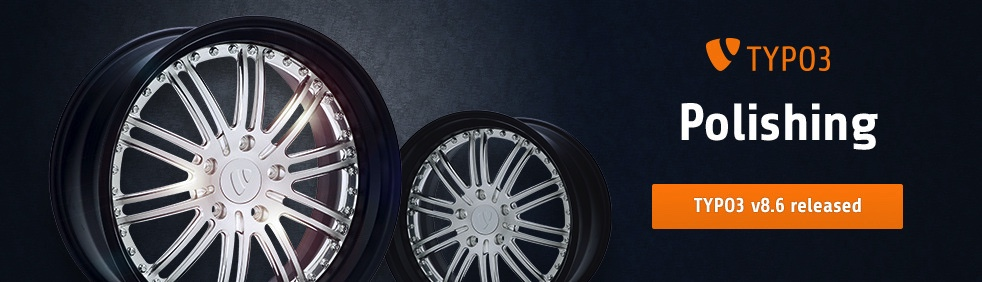
\includegraphics[width=0.95\linewidth]{Introduction/typo3cms86-banner.jpg}
	\end{figure}

\end{frame}

% ------------------------------------------------------------------------------
% LTXE-SLIDE-START
% LTXE-SLIDE-UID:		8dac05aa-4b4ae956-a25fc943-c2ada9ea
% LTXE-SLIDE-ORIGIN:	edf38742-589c1a34-ae855361-e0284741 English
% LTXE-SLIDE-TITLE:		System Requirements
% ------------------------------------------------------------------------------
\begin{frame}[fragile]
	\frametitle{Inleiding}
	\framesubtitle{Systeemeisen}

	\begin{itemize}
		\item PHP:\tabto{2.2cm}versie 7
		\item MySQL:\tabto{2.2cm}versie 5.5 tot 5.7
		\item Schijfruimte:\tabto{2.2cm}min 200 MB
		\item PHP-instellingen:

			\begin{itemize}
				\item \texttt{memory\_limit} >= 128M
				\item \texttt{max\_execution\_time} >= 240s
				\item \texttt{max\_input\_vars} >= 1500
				\item compilatieoptie \texttt{-}\texttt{-disable-ipv6} \underline{niet} gebruiken
			\end{itemize}

		\item De backend vereist Microsoft Internet Explorer 11 of hoger,
			Microsoft Edge, Google Chrome, Firefox, Safari
			of een andere moderne, compatibele browser

	\end{itemize}

\end{frame}

% ------------------------------------------------------------------------------
% LTXE-SLIDE-START
% LTXE-SLIDE-UID:		afd5634e-fc9b6110-9b8b893e-6f85f062
% LTXE-SLIDE-ORIGIN:	8cb2705f-d045b3fa-b2ca4f81-52d16aef English
% LTXE-SLIDE-TITLE:		Development And Release Timeline
% ------------------------------------------------------------------------------
\begin{frame}[fragile]
	\frametitle{Inleiding}
	\framesubtitle{Ontwikkelings- en publicatietijdlijn}

	\begin{figure}
		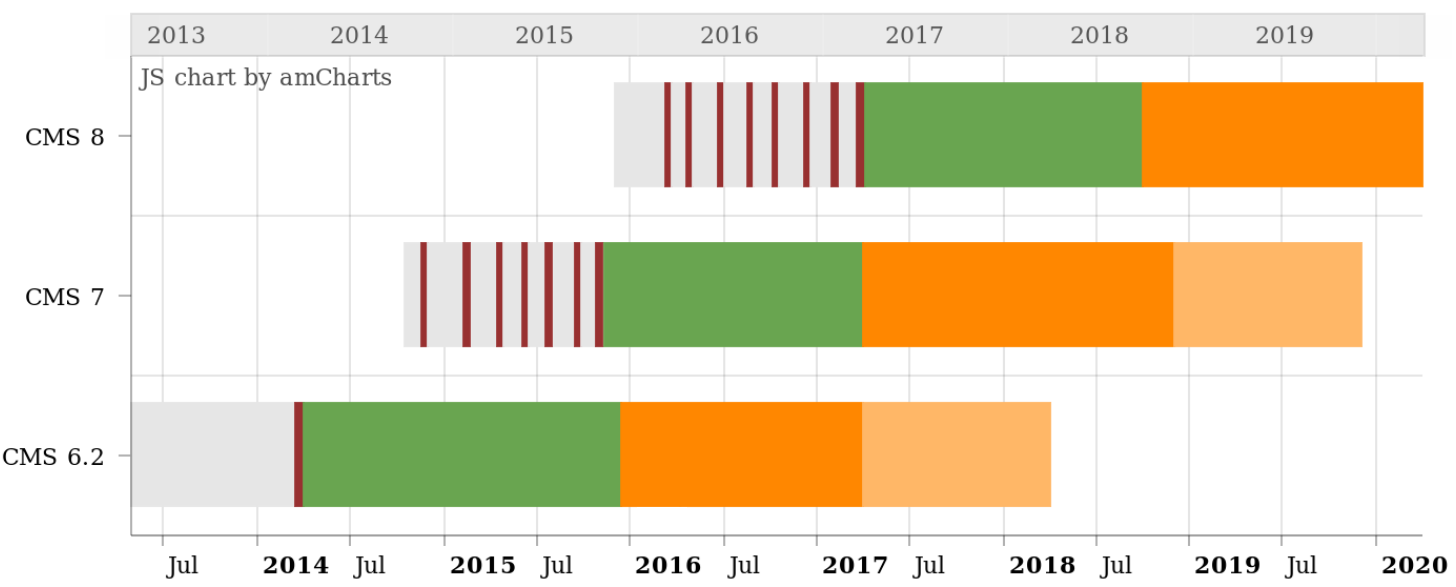
\includegraphics[width=1\linewidth]{Introduction/ReleaseAgenda.png}
	\end{figure}

\end{frame}

% ------------------------------------------------------------------------------
% LTXE-SLIDE-START
% LTXE-SLIDE-UID:		3d7bd26e-ec357470-0c1b2277-1d00b487
% LTXE-SLIDE-ORIGIN:	dae3f732-e4550c37-dc304056-f090affc English
% LTXE-SLIDE-TITLE:		TYPO3 CMS Roadmap
% ------------------------------------------------------------------------------
\begin{frame}[fragile]
	\frametitle{Inleiding}
	\framesubtitle{TYPO3 CMS Roadmap}

	Publicatiedatums en de primaire focus:

	\begin{itemize}

		\item v8.0 \tabto{1.1cm}22 mar 2016\tabto{3.4cm}Lastminute toevoegingen
		\item v8.1 \tabto{1.1cm}03 mei 2016\tabto{3.4cm}Cloud-integratie
		\item v8.2 \tabto{1.1cm}05 jul 2016\tabto{3.4cm}Randvoorwaarden Doctrine
		\item v8.3 \tabto{1.1cm}30 aug 2016\tabto{3.4cm}Rich Text Editor
		\item v8.4 \tabto{1.1cm}18 okt 2016\tabto{3.4cm}Doctrine-migratie + upgrades
		\item v8.5 \tabto{1.1cm}20 dec 2016\tabto{3.4cm}Nieuwe RTE + Integrator-ondersteuning
		\item
			\begingroup
				\color{typo3orange}
					v8.6 \tabto{1.1cm}14 feb 2017\tabto{3.4cm}Polijsten
			\endgroup
		\item v8.7 \tabto{1.1cm}04 apr 2017\tabto{3.4cm}Voorbereiding LTS

	\end{itemize}

	\smaller
		\url{https://typo3.org/typo3-cms/roadmap/}\newline
		\url{https://typo3.org/news/article/kicking-off-typo3-v8-development/}
	\normalsize

\end{frame}

% ------------------------------------------------------------------------------
% LTXE-SLIDE-START
% LTXE-SLIDE-UID:		aba51f2f-5cd78ccc-a77b0a12-76636ac6
% LTXE-SLIDE-ORIGIN:	4a382358-6fd84263-041bc029-bd50bb1e English
% LTXE-SLIDE-TITLE:		Installation
% ------------------------------------------------------------------------------
\begin{frame}[fragile]
	\frametitle{Inleiding}
	\framesubtitle{Installatie}

	\begin{itemize}
		\item Officiële \textit{klassieke} installatieprocedure op Linux/Mac OS X\newline
			(DocumentRoot bijvoorbeeld \texttt{/var/www/site/htdocs}):
		\begin{lstlisting}
			$ cd /var/www/site
			$ wget --content-disposition get.typo3.org/8.6
			$ tar xzf typo3_src-8.6.0.tar.gz
			$ cd htdocs
			$ ln -s ../typo3_src-8.6.0 typo3_src
			$ ln -s typo3_src/index.php
			$ ln -s typo3_src/typo3
			$ touch FIRST_INSTALL
		\end{lstlisting}

		\item Symbolische koppelingen op Microsoft Windows:

			\begin{itemize}
				\item Gebruik \texttt{junction} op Windows XP/2000
				\item Gebruik \texttt{mklink} op Windows Vista en Windows 7
			\end{itemize}

	\end{itemize}
\end{frame}

% ------------------------------------------------------------------------------
% LTXE-SLIDE-START
% LTXE-SLIDE-UID:		789eab54-60e35535-3a5afcf5-46a494b7
% LTXE-SLIDE-ORIGIN:	db02b644-4eae727a-2eff0fa0-9cbd7fd3 English
% LTXE-SLIDE-TITLE:		Upgrade to TYPO3 CMS 7
% ------------------------------------------------------------------------------
\begin{frame}[fragile]
	\frametitle{Inleiding}
	\framesubtitle{Upgrade naar TYPO3 CMS 8.x}

	\begin{itemize}
		\item Upgrades alleen mogelijk vanaf TYPO3 CMS 7.6 LTS
		\item TYPO3 CMS < 7.6 LTS moet eerst naar TYPO3 CMS 7.6 LTS bijgewerkt worden
	\end{itemize}

	\begin{itemize}

		\item Instructies voor het upgraden:\newline
			\smaller\url{http://wiki.typo3.org/Upgrade#Upgrading_to_8.6}\normalsize
		\item Officiële TYPO3-handleiding "TYPO3 Installation and Upgrading":
			\smaller\url{http://docs.typo3.org/typo3cms/InstallationGuide}\normalsize
		\item Algemene aanpak:
			\begin{itemize}
				\item Controleer minimale systeemeisen \small(PHP, MySQL, etc.)
				\item Controleer \textbf{deprecation\_*.log} in de oude TYPO3-installatie
				\item Werk alle extensies bij naar de nieuwste versie
				\item Plaats nieuwe broncode en start Installatie-module \textrightarrow Upgrade Wizard
				\item Controleer de startmodule voor backend gebruikers (optioneel)
			\end{itemize}
	\end{itemize}

\end{frame}

% ------------------------------------------------------------------------------

% ------------------------------------------------------------------------------
% LTXE-SLIDE-START
% LTXE-SLIDE-UID:		2f336d5a-204b1c99-b0bbecd7-35b7aec8
% LTXE-SLIDE-ORIGIN:	d9a72263-ac0c63dd-1754b138-99b8491c English
% LTXE-SLIDE-TITLE:		PHP Version 7
% ------------------------------------------------------------------------------
\begin{frame}[fragile]
	\frametitle{Inleiding}
	\framesubtitle{PHP Versie 7}

	\begin{itemize}

		\item TYPO3 CMS 8.x vereist minimaal PHP 7.0
		\item TYPO3 zal volgende PHP 7-versies ondersteunen
		\item Deze versie geeft significant betere prestaties op het hele systeem

		\item Niet alleen backendgebruikers ervaren een soepelere interface: het
			nieuwe record voor het laden van een volledig gecachete pagina in de frontend is nu minder
			dan 7 milliseconden, wat ongeveer 40\% sneller is dan met PHP versie 5.5

		\item We zijn reeds begonnen met het gebruiken van nieuwe kenmerken van deze PHP-versie,
			de cryptografisch veilige pseudotoevalsgeneratoren worden bijvoorbeeld al ingezet

	\end{itemize}

\end{frame}

% ------------------------------------------------------------------------------
